\documentclass[16pt]{report}
\input{preamble.tex}
\usepackage[scr]{rsfso}


\title{\Huge{Structure Discrète}\\{IFT1065}\\{\textbf{Concepts de logique}}}
\author{\huge{Franz Girardin}}
\date{2 Octobre 2023}
\lstset{inputencoding=utf8/latin1}

            %%%%%%%%%%%%%%%%%  Sect.                          %%%%%%%%%%%%%%%%%%%%%%%%%%%%%%%%%%%%%%%%%%%%%%%%%%%%%%%%%
\usepackage{helvet}
\titleformat{\chapter}
  {\fontfamily{phv}\bfseries\huge} % format
  {}                % label
  {0pt}             % sep
  {\color{myb}\huge}           % before-code



\titleformat{\section}
  {\normalfont\scshape}{\thesection}{1em}{}


% Customizing the spacing for the chapter titles
\titlespacing*{\chapter}{0pt}{0pt}{20pt}

\usepackage{mathpazo}
\begin{document}
\maketitle
\pagebreak
\tableofcontents 
\pagebreak

\pagebreak
\begin{multicols*}{2}
        \chapter{Introduction à la logique}
        \section{Concept de logique et proposition}
                La logique est une façon de raisonner. Simplement, elle permet de \textbf{déduire} de nouvelles
                informations à partir d'information antérieure, tout en déterminant le sens de ce qui a été évoqué à 
                travers l'information.

        \begin{Definitionx}{Proposition}{}
            Une proposition est une \textbf{phrase} ou une \textbf{expression mathématique} qui est soit 
            définitivement vraie ou définitivement fausse. 
        \end{Definitionx}


        \begin{EExample}{Proposition}{}
                \begin{enumerate}
                    \item $S : \{0, -1, -2 \} \cap \mathbb{N} = \emptyset$ est un proposition \textbf{vraie} \\ 
                \end{enumerate}
        \end{EExample}


                Les propositions peuvent contenir des variables. Par exemple, 
                « \textbf{$P(x) : \text{ Soit un entier } x, \; x^2 \text{ sera toujours positif} $} » est 
                une \textcolor{red}{proposition contenant une variable} et cette proposition est vraie. 
                Par contre, une phrase contenant une variable n'est pas nécessairement un proposition :
                « $Q(x) : \text{L'entier } x \text{ est pair}$ » n'est ni définitivement vrai, ni définitivement 
                faux; cela dépendra de la valeur de $x$. Ainsi, $Q(x)$ \textbf{n'est pas} un proposition.   

        \begin{Definitionx}{Phrase ouverte}{}
            Une phrase ouverte est une phrase telle que sa véracité dépend d'un contexte. 
        \end{Definitionx}
        %%%%%%%%%%%%%%%%%  Sect.  AND OR NOT                 %%%%%%%%%%%%%%%%%%%%%%%%%%%%%%%%%%%%%%%%%%%%%%%%%%%%%%%%%%
        

        \section{Opérateurs logiques}
                On peut utiliser le mot « \textbf{et} » pour combiner deux propositions ; cela engendre une 
                \textbf{nouvelle proposition}. 
                \begin{Syntaxe}{Opérateur logique $\land$ }{}
                   Soit les propositions $P, Q$ et la proposition $R = P \land Q$ ; $R$ est \textbf{vraie} si 
                   et seulement si à la fois $P$ et $Q$ sont vrais. 
                \end{Syntaxe}
                
                
                \begin{table}[H]
                  \caption {Table de vérité de $P \land Q$}
                  \begin{center}
                   \renewcommand{\arraystretch}{1.5}
                   \fontfamily{flr}\selectfont
                    \normalsize
                        \begin{tabular}{|l|l||l|}
                        \arrayrulecolor{blue}\hline
                        \rowcolor{lightBlue}
                        \textcolor{myb}{$P$} & \textcolor{myb}{$Q$} & \textcolor{myb}{$P \land Q$}   
                        \\
                        \hline
                        \hline
                        \arrayrulecolor{black}
                        $V$ & $V$ & \cellcolor{myg} $V$
                        \\
                        \hline
                        $V$ & $F$ & \cellcolor{myr} $F$ 
                        \\
                        \hline
                        $F$ & $V$ & \cellcolor{myr} $F$ 
                        \\
                        \hline 
                        $F$ & $F$ & \cellcolor{myr} $F$ 
                        \\ 
                        \hline
                        \end{tabular}
                \end{center}
                \end{table}


                On peut utiliser le mot « \textbf{ou} » pour combiner deux propositions ; cela engendre une 
                \textbf{nouvelle proposition}. 
                \begin{Syntaxe}{Opérateur logique $\lor$ }{}
                   Soit les propositions $P, Q$ et la proposition $R = P \lor Q$ ; $R$ est \textbf{vraie} si 
                   au moins $P$ ou $Q$ est vraie. 
                \end{Syntaxe}

                \begin{table}[H]
                  \caption {Table de vérité de $P \lor Q$}
                  \begin{center}
                   \renewcommand{\arraystretch}{1.5}
                   \fontfamily{flr}\selectfont
                    \normalsize
                        \begin{tabular}{|l|l||l|}
                        \arrayrulecolor{blue}\hline
                        \rowcolor{lightBlue}
                        \textcolor{myb}{$P$} & \textcolor{myb}{$Q$} & \textcolor{myb}{$P \lor Q$}   
                        \\
                        \hline
                        \hline
                        \arrayrulecolor{black}
                        $V$ & $V$ & \cellcolor{myg} $V$
                        \\
                        \hline
                        $V$ & $F$ & \cellcolor{myg} $V$ 
                        \\
                        \hline
                        $F$ & $V$ & \cellcolor{myg} $V$ 
                        \\
                        \hline 
                        $F$ & $F$ & \cellcolor{myr} $F$ 
                        \\ 
                        \hline
                        \end{tabular}
                \end{center}
                \end{table}



                On peut utiliser l'expression « \textbf{il n'est pas vrai que} » devant une propositions ; 
                cela engendre une \textbf{nouvelle proposition}. 
                \begin{Syntaxe}{Opérateur logique $\neg$ }{}
                   Soit la propositions $P$ et la proposition $Q = \neg P$ ; $P$ est \textbf{vraie} si 
                   et seulement si $Q$ n'est pas vrai, \textbf{et vice versa}.
                \end{Syntaxe}



                \begin{table}[H]
                  \caption {Table de vérité de $ \neg P$}
                  \begin{center}
                   \renewcommand{\arraystretch}{1.5}
                   \fontfamily{flr}\selectfont
                    \normalsize
                        \begin{tabular}{|l||l|}
                        \arrayrulecolor{blue}\hline
                        \rowcolor{lightBlue}
                        \textcolor{myb}{$P$} & \textcolor{myb}{$\neg P$} 
                        \\
                        \hline
                        \hline
                        \arrayrulecolor{black}
                        $V$ & \cellcolor{myr} $F$
                        \\
                        \hline 
                        $F$ & \cellcolor{myg} $V$ 
                        \\ 
                        \hline
                        \end{tabular}
                \end{center}
                \end{table}


                \section{Propositions conditionnelles}



                On peut utiliser l'expression « \textbf{si..., alors...} » entre deux propositions ; cela engendre une 
                \textbf{nouvelle proposition}. 
                \begin{Syntaxe}{Opérateur logique $\implies$ }{}
                    Soit la propositions $P$ et la proposition $Q$ ; 
                    \[ R = P \implies  Q \] 
                    indique que $R$ est \textbf{vraie} si 
                    le fait que $P$ est vraie \textbf{implique nécessairement} que $Q$ soit vraie. Il s'agit d'une 
                    proposition conditionnelle, puisque $Q$ sera vraie \textbf{sous la condition} que $P$ soit vraie.  
                \end{Syntaxe}


            \begin{table}[H]
            \caption {Table de vérité de $P \implies Q$}
                  \begin{center}
                   \renewcommand{\arraystretch}{1.5}
                   \fontfamily{flr}\selectfont
                    \normalsize
                        \begin{tabular}{|l|l||l|}
                        \arrayrulecolor{blue}\hline
                        \rowcolor{lightBlue}
                        \textcolor{myb}{$P$} & \textcolor{myb}{$Q$} & \textcolor{myb}{$P \implies Q$}   
                        \\
                        \hline
                        \hline
                        \arrayrulecolor{black}
                        $V$ & $V$ & \cellcolor{myg} $V$
                        \\
                        \hline
                        $V$ & $F$ & \cellcolor{myr} $F$ 
                        \\
                        \hline
                        $F$ & $V$ & \cellcolor{myg} $V$ 
                        \\
                        \hline 
                        $F$ & $F$ & \cellcolor{myg} $V$ 
                        \\ 
                        \hline
                        \end{tabular}
                \end{center}
            \end{table}

            \section{Proposition Biconditionnelle}
            \begin{note}{}{}
                Les proposition suivantes ne sont pas équivalentes 
                \[ P \implies  Q  \neq Q \implies P \]  
                D'ailleurs, on dit que l'une est la \textcolor{red}{\textit{réciproque}} de l'autre     
            \end{note} 
            

                Deux propositions $P$ et $Q$ peuvent être telles que $Q$ est la réciproque de $P$ et les 
                deux sont à la fois vrai. Puisque ces deux propositions sont vraies, leur conjonction est aussi vraie 
                On obtient alors : 
                \[ (P \implies Q) \land (Q \implies P) \;\; \textcolor{myg}{Vraie}  \]
                Nous introduisons alors un nouveau symbole qui illustre la relation entre $P$ et $Q$ ; la conjonction 
                suivante engendre une proposition \textcolor{red}{\textit{biconditionnelle}} : 
                \begin{enumerate}
                    \item $Q \implies P$ « \textit{P si Q} »
                    \item $P \implies Q$ « \textit{P seulment si Q} » \\
                    \item $ P \Leftrightarrow  Q \equiv (P \implies Q) \land (Q \implies P)$  
                    \item $ P \Leftrightarrow  Q $ « \textit{P si et seulement si Q} » 
                \end{enumerate}

            
 
            \begin{table}[H]
            \caption {Table de vérité de $P \Leftrightarrow Q$}
                  \begin{center}
                   \renewcommand{\arraystretch}{1.5}
                   \fontfamily{flr}\selectfont
                    \normalsize
                        \begin{tabular}{|l|l||l|}
                        \arrayrulecolor{blue}\hline
                        \rowcolor{lightBlue}
                        \textcolor{myb}{$P$} & \textcolor{myb}{$Q$} & \textcolor{myb}{$P \Leftrightarrow Q$}   
                        \\
                        \hline
                        \hline
                        \arrayrulecolor{black}
                        $V$ & $V$ & \cellcolor{myg} $V$
                        \\
                        \hline
                        $V$ & $F$ & \cellcolor{myr} $F$ 
                        \\
                        \hline
                        $F$ & $V$ & \cellcolor{myr} $F$ 
                        \\
                        \hline 
                        $F$ & $F$ & \cellcolor{myg} $V$ 
                        \\ 
                        \hline
                        \end{tabular}
                \end{center}
            \end{table}
            
            La proposition biconditionnelle indique que soit les deux propositions qui la composent sont soit toutes 
            deux vraies, ou elles sont soit toutes deux fausses.


            \section{Table de vérité de propositions}
            Considérons un problème plus complexe où une expression impliques plusieurs propositions combinées. 
            Nous allons essayer déterminer pour quelles valeurs de $P$ et $Q$ une proposition complexe $R$ est vraie. 
            \[ Soit \; R = (P \lor Q)\land \neg (P \land Q)\]
            $R$ indique que \textit{P ou Q est vraie et il n'est pas possible que P et Q soient vrai à la fois}.


            \begin{table}[H]
                \caption{Table de vérité pour $(P \lor Q) \land \neg (P \land Q)$}
                \begin{center}
                \renewcommand{\arraystretch}{1.5}
                \fontfamily{flr}\selectfont
                \footnotesize
            \begin{tabular}{|l|l||l|l|l||l|}
                    \arrayrulecolor{blue}\hline
                    \rowcolor{lightBlue}
                    \textcolor{myb}{$P$} & \textcolor{myb}{$Q$} & \textcolor{myb}{$(P \lor Q)$} & 
                    \textcolor{myb}{$P \land Q$)} & \textcolor{myb}{$\neg (P \land Q)$} & 
                    \textcolor{myb}{$(P \lor Q) \land \neg (P \land Q)$}
                    \\
                    \hline
                    \hline
                    \arrayrulecolor{black}
                    \cellcolor{myg} $T$ & \cellcolor{myg} $T$ & \cellcolor{myg} $T$ &
                    \cellcolor{myg} $T$ & \cellcolor{myr} $F$ & \cellcolor{myr} $F$ 
                    \\
                    \hline
                    \cellcolor{myg} $T$ & \cellcolor{myr} $F$ & \cellcolor{myg} $T$ & 
                    \cellcolor{myr} $F$ & \cellcolor{myg} $T$ & \cellcolor{myg} $T$ 
                    \\ 
                    \hline 
                    \cellcolor{myr} $F$ & \cellcolor{myg} $T$ & \cellcolor{myg} $T$ &
                    \cellcolor{myr} $F$ & \cellcolor{myg} $T$ & \cellcolor{myg} $T$ 
                    \\ 
                    \hline
                    \cellcolor{myr} $F$ & \cellcolor{myg} $F$ & \cellcolor{myr} $F$ &
                    \cellcolor{myr} $F$ & \cellcolor{myg} $T$ & \cellcolor{myr} $F$
                    \\ 
                    \hline
                    \end{tabular}
            \end{center}
            \end{table}
        
            %%%%%%%%%%%%%%%%%  Sect. Équivalences logiques  %%%%%%%%%%%%%%%%%%%%%%%%%%%%%%%%%%%%%%%%%%%%%%%%%%%%%%%%%%%

            
            \section{Équivalences logiques}
            \begin{Definitionx}{Notion d'équivalence logique}{}
                    Deux propositions sont dite \textbf{logiquement équivalentes} si leurs valeurs correspondent 
                    exactement dans une table de vérité.
            \end{Definitionx}


                    En utilisant une table de vérité, on peut montrer que les propositions suivantes sont 
                    logiquement équivalentes. 
                    \begin{enumerate}
                        \item $ P \Leftrightarrow  Q = (P \land Q) \lor (\neg P \land \neg Q )$ 
                        \item $ P \implies Q = \neg P \implies \neg Q$  
                    \end{enumerate}



            \begin{table}[H]
                \caption{Table de vérité pour $ P \implies Q = \neg P \implies \neg Q$}
                \begin{center}
                \renewcommand{\arraystretch}{1.5}
                \fontfamily{flr}\selectfont
                \footnotesize
            \begin{tabular}{|l|l||l|l|l||l|}
                    \arrayrulecolor{blue}\hline
                    \rowcolor{lightBlue}
                    \textcolor{myb}{$P$} & \textcolor{myb}{$Q$} & \textcolor{myb}{$\neg P$} & 
                    \textcolor{myb}{$\neg Q$)} & \textcolor{myb}{$\neg P \implies \neg Q$} & 
                    \textcolor{myb}{$P \implies  Q$}
                    \\
                    \hline
                    \hline
                    \arrayrulecolor{black}
                    \cellcolor{myg} $V$ & \cellcolor{myg} $V$ & \cellcolor{myr} $F$ &
                    \cellcolor{myr} $F$ & \cellcolor{myg} $V$ & \cellcolor{myg} $V$ 
                    \\
                    \hline
                    \cellcolor{myg} $V$ & \cellcolor{myr} $F$ & \cellcolor{myr} $F$ & 
                    \cellcolor{myg} $V$ & \cellcolor{myr} $F$ & \cellcolor{myr} $F$ 
                    \\ 
                    \hline 
                    \cellcolor{myr} $F$ & \cellcolor{myg} $V$ & \cellcolor{myg} $V$ &
                    \cellcolor{myg} $V$ & \cellcolor{myg} $V$ & \cellcolor{myg} $V$ 
                    \\ 
                    \hline
                    \cellcolor{myr} $F$ & \cellcolor{myr} $F$ & \cellcolor{myg} $V$ &
                    \cellcolor{myg} $V$ & \cellcolor{myg} $V$ & \cellcolor{myg} $V$
                    \\ 
                    \hline
                    \end{tabular}
            \end{center}
            \end{table} 


            
            %%%%%%%%%%%%%%%%%  Sect. Loi DeMorgan           %%%%%%%%%%%%%%%%%%%%%%%%%%%%%%%%%%%%%%%%%%%%%%%%%%%%%%%%%%%

            \section{DeMorgan} 
            \begin{Concept}{Loi DeMorgan}{}
                \begin{enumerate}
                    \item $\neg (P \land Q) = (\neg P) \lor (\neg Q)$
                    \item $\neg (P \lor Q) = (\neg P) \land (\neg Q)$
                \end{enumerate}
            \end{Concept}
                    
                    La loi DeMorgan est intuitive. Affirmer $\neg (P \land Q)$ revient à dire qu'il n'est pas 
                    possible que $P$ et $Q$ soient vrais à la fois. Or, si $P$ et $Q$ ne peuvent pas être 
                    tout deux vrai, soit $P$ est faux, $ \neg P$, ou aors $Q$ est faux, $\neg Q$.


            Nous résumons ici quelques équivalences logiques importantes. 
            \begin{itemize}
                \item Loi de la contraposé 
                    \begin{enumerate}
                        \item $P \implies Q = \neg Q \implies \neg P$ 
                    \end{enumerate}
                \item Loi DeMorgan
                    \begin{enumerate}
                        \item $\neg (P \land Q) = (\neg P) \lor (\neg Q)$ 
                        \item $\neg (P \lor Q) = (\neg P) \land (\neg Q)$
                    \end{enumerate}
                \item Loi commutative
                    \begin{enumerate}
                        \item $P \land Q = Q \land P$ 
                        \item $P \lor Q = Q \lor P$ 
                    \end{enumerate}
                \item Loi distributive
                    \begin{enumerate}
                        \item $ P \land (Q \lor R) = (P \land Q) \lor (P \land R) $
                        \item $ P \lor (Q \land R) = (P \lor Q) \land (P \land R)$ 
                    \end{enumerate}    
                \item Loi associative
                    \begin{enumerate}
                    \item $P \land (Q \land R) = (P \land Q) \land R = P \land Q \land R$ 
                    \item $P \lor (Q \lor R) = (P \lor Q) \lor R = P \lor Q \lor R$
                    \end{enumerate}
            \end{itemize}


            %%%%%%%%%%%%%%%%%  Sect. Propositions quantitifées %%%%%%%%%%%%%%%%%%%%%%%%%%%%%%%%%%%%%%%%%%%%%%%%%%%%%%%%
            
\chapter{Propositions Quantifiées}

            \section{Introduction aux quatificateurs}
            Certaines propositions peuvent difficilement être symbolisé par un nombre limité 
            \textbf{d'opérateurs} logique. Considérons l'ensemble infini d'entiers $S = \{x_1, x_2, x_3, \dots \}$.
            Pour exprimer l'affirmation \textit{chaque élément de S est impair}, il faudrait procéder 
            de la façon suivante : 
            \[ P(x_1) \land P(x_2) \land P(x_3) \land \dots \]
            Noton ici que $P(x)$ est la phrahse ouverte \textit{x est impair}.  
            Néanmoins, cette approche engendre une expression interminable. Similairement, pour exprimer la proposition 
            selon laquelle \textit{il y a au moins un élément de S qui est impair}, on aurait 
            procéder de la façon suivante : 
            \[ P(x_1) \lor P(x_2) \lor P(x_3) \lor \dots \]
            
            
            \begin{Concept}{}{}
                Nous itroduisons le symbole $\forall$ qui signifie \textit{pour tout}, et le symbole 
                $\exists$ qui signifie \textit{il existe}.   
            \end{Concept}
            
            Nous pouvons réécrire les deux expression précédentes de la façon suivante : 
            \begin{enumerate}
                \item $\forall x \in S, \;\; P(x)$ 
                \item $\exists x \in S, \;\; P(x)$  
            \end{enumerate}


            \begin{note}{}{}
                $\forall$ est appelé \textit{quantificateur universel} et $\exists$ est appelé 
                \textit{quantificateur existentiel}. Les propositions qui contiennent l'un ou l'autre sont appeléss 
                \textit{proposition quantifiées}. 
            \end{note} 
            

            \section{Quantificateur implicite}
            \begin{Concept}{Quantificateur implicite}{}
                En mathématique, lorsque $P(x)$ et $Q(x)$ sont des phrases ouvertes concernant un élément $x$ 
                appartenant à un certain ensemble $S$, une expression de la forme $P(x) \implies  Q(x)$ 
                est comprise comme étant implicitement $\forall x \in S, P(x) \implies  Q(x)$. L'omission du 
                $\forall x \in S$ est un convention. Ce type d'expression revient souvent et on préfère éviter de 
                répéter la portion quantificatrice de l'expression. 
            \end{Concept}

           \begin{Definitionx}{}{}
               Si $P$ et $Q$ sont des proposition ou des phrases ouverte, 
               \[ Si \; P, \; alors \; Q\]
               est une proposition. 
           \end{Definitionx}
            \section{Interchangeabilité de l'universellement et de la proposition conditionnelle}
           \begin{EExample}{Conjecture de Golbach}{}
               La conjecture de Golbach indique que 
               \textit{chaque entier plus grand que 2 est la somme de deux nombres premiers}. Nous pouvons traduire 
               cette proposition de la façon suivante : 
               \begin{itemize}
                   \item Soit  $S = \{ x \;|\; x \geq 2\}$
                       \begin{enumerate}
                        \item $(n \in S) \implies  (\exists p, q \in P, n = p + q)$ 
                        \item $\forall n \in S, \exists p, q \in P, n = p + q$ 
                       \end{enumerate}
               \end{itemize}
           \end{EExample}



           \begin{Theorem}{}{}
               Suppopsons que $S$ est un ensemble et $Q(x)$ est une proposition par rapport à $x$ pour 
               n'importe quel $x \in S$. Nous savons alors que les deux propositions suivantes veulent dire 
               la même chose 
               \begin{enumerate}
                \item $\forall x \in S, Q(x)$
                \item  $x \in S \implies  Q(x)$
               \end{enumerate}
           \end{Theorem}

            

           \section{Négation de proposition}
            Soit une proposition $R$, la proposition $\neg R$ est la négation de $R$. Certaines expressions sont 
            plus utiles sous leur forme négative. Le processus pour trouver $-R$ est la \textbf{négation de $R$}  
        
    
            \begin{EExample}{Négation d'une proposition}{}
                Soit la proposition 
                \begin{itemize}
                    \item $R$ :
                    \textit{Tu peux résoudre le problème en factorisant ou en utilisant le fomule quadratique }.
                    \begin{enumerate}
                        \item $P = \textit{Tu peux résoudre le problème en factorisant}$ 
                        \item $Q = \textit{...avec la formule quadratique}$. 
                        \item On a : 
                             \[ \neg R = \neg (P \lor Q) \]
                             \[ \neg R = \neg(P) \land \neg(Q) \] 
                    \end{enumerate}
                \end{itemize} 
            \end{EExample} 

            %%%%%%%%%%%%%%%%%  Sect. Negation propositions quantitifées  %%%%%%%%%%%%%%%%%%%%%%%%%%%%%%%%%%%%%%%%%%%%%%


            \section{Négation de proposition quantitifée} 

            Considérons une proposition quantitifée : 
            \[ R = \forall x \in \mathbb{N}, P(x)\]
            La négation de cette proposition est : 
            \textit{ce n'est pas le cas que pour tout x dans $\mathbb{N} \; P(x)$ est vrai}. Autrement dit, 
            \textit{il existe un $x$ dans $\mathbb{N}$ tel que $P(x)$ est faux}. Nous pouvons traduire la négation 
            de $R$ de la façon suivante : 
            \[ \neg R = \exists x \in \mathbb{N}, \neg P(x) \]
            Nous constatons que la négation d'une proposition universellement quantitifées engendre une 
            proposition existantielle. La réciproque est aussi vraie. 


            \begin{Theorem}{Négation de proposition universellement ou existentiellement quantitifée}{}
                \[ \neg (\forall x \in S, P(x) = \exists x \in S, \neg P(x))\]
                \[ \neg (\exists x \in S, P(x) = \forall x \in S, P(x)) \]
            \end{Theorem}

            \section{Négation de proposition ayant plusieurs quantificateurs}
            Lorsqu'un proposition présente plusieurs quantificateurs, il faut décomposer le sens de l'expression 
            itérativement. 
            
            \begin{EExample}{Négation de proposition à plusieurs quantificateurs}{}
                Soit la proposition 
                \begin{itemize}
                    \item $S$ : \textit{pour tout nombre réel $x$, il existe un nombre réel $y$ pour lequel $y^3 = x$} 
                        \begin{enumerate}
                            \item $ S = \forall x \in \mathbb{R}, \exists y \in \mathbb{R}, y^3 = x$ 
                            \item $ \neg S = \neg (\forall x \in \mathbb{R}, \exists y \in \mathbb{R}, y^3 = x)$
                            \item  $\neg S = \neg (\forall x \in \mathbb{R}), \forall y \in \mathbb{R}, y^3 \neq x$ 
                            \item  $\neg S = \exists x \in \mathbb{R}, \forall y \in \mathbb{R}, y^3 \neq x$
                        \end{enumerate}
                    \item $ \neg S$ : \textit{il existe un réel $x$ tel que pour tout réel $y$, $y^3 \neq x$}

                \end{itemize}
            \end{EExample}


            \section{Négation de proposition conditionnelle}
            Nous savons que la proposition conditionnelle $P \implies  Q$ est fausse uniquement lorsque $P$ est vraie, 
            mais que $Q$ est faux. Ainsi, nous avons : 
            \[ \neg P \implies  Q = P \land \neg Q \]

            \begin{EExample}{Négation d'une proposition conditionnelle}{}
                Soit la proposition
                \begin{itemize}
                    \item  $R = \textit{Si  $x$ est impair, $x^2$ est impair}$  
                        \begin{enumerate}
                            \item $\neg R = \neg \Bigl(\forall x \in \mathbb{Z}, 
                                (x \; est \; impair) \implies  x^2 \; est \; impair\Bigr)$
                            \item $\neg R = \exists x \in \mathbb{Z}, 
                                (x \; est \; impair) \implies  \neg (x^2 \; est \;  impair)$ 
                        \end{enumerate}
                \end{itemize}

            \end{EExample}




                        %%%%%%%%%%%%%%%%%  Sect. Techniques de preuve    %%%%%%%%%%%%%%%%%%%%%%%%%%%%%%%%%%%%%%%%%%%%%%%
            
            \chapter{Techniques de preuve}
            

            \section{Définitions de termes récurrents} 


            \begin{Definitionx}{Définir un théorème}{}
                        Est un \textbf{théorème} une proposition mathématique qui est vraie et peut être vérifiée comme 
                        étant vraie. Une \textbf{preuve} d'un théorème est une vérification écrite qui montre que le 
                        théorème est, sans équivoque, vrai. Une \textbf{définition} est une explication exacte et 
                        non ambigue d'une expression mathématique. 
            \end{Definitionx}                                                                                            
            
            \begin{Definitionx}{Lemme}{}
                        Il s'agit d'un théorème mineur dont l'objectif est d'aider à montrer la véracité d'un autre 
                        théorème. 
            \end{Definitionx}

            \begin{Definitionx}{Corollaire}{}
                        Il s'agit d'un résultat qui est la conséquence directe d'un autre théorème ou d'une 
                        autre proposition. 
            \end{Definitionx}


            %%%%%%%%%%%%%%%%%  Sect. Définitions d'entités mathématiques%%%%%%%%%%%%%%%%%%%%%%%%%%%%%%%%%%%%%%%%%%%%%%%
            \pagebreak
            \section{définition d'entités mathématiques}

            \begin{itemize}
                \item \textcolor{myp}{\textbf{Pair et impair}} 
                    \begin{enumerate}
                        \item Un \textbf{entier} $n$ est \textbf{\textcolor{myb}{pair}} si $n = 2a$ 
                    pour un certain entier $a \in Z$
                        \item Un \textbf{entier} $n$ est \textbf{\textcolor{myb}{impair}} si $n = 2a + 1$ 
                    pour un certain entier $a \in Z$
                    \end{enumerate}

                \item Deux entiers ont \textbf{\textcolor{myb}{la même parité}} s'ils sont tous deux 
                    \textbf{pairs} ou tout deux \textbf{impairs}. 
                    Autrement, ils ont une \textbf{\textcolor{myb}{parité opposée}}. 
                \item \textcolor{myp}{\textbf{Division et multiplication}}

                \begin{enumerate}
                    \item \textcolor{myb}{\textbf{Division}}. Soit les entier $a$ et $b$. On dit que 
                        $a$ \textbf{\textcolor{myb}{divise}} $b$ si $b = ac$, pour un certain entier $c \in \mathbb{Z}$.
                        On écrit $a$ divise $b$ : $a | b$
                    \item \textcolor{myb}{\textbf{Multiplication}}. On dit également que $a$ est un 
                        \textcolor{myb}{\textbf{diviseur}}   de $b$ et que $b$ est un 
                        \textbf{\textcolor{myb}{multiple}} de $a$.
                    \item Lorsque $a$ \textcolor{myb}{\textbf{ne divise pas}} $b$, on écrit $a \nmid b$. 
                \end{enumerate}

                \item \textbf{\textcolor{myp}{Nombre premier}}
                    \begin{enumerate}
                        \item Chaque  \textbf{entier} a un ensemble d'entiers qui peuvent le diviser. Par exemples,
                            les diviseur de $6$ sont dans l'ensemble 
                            \[ \{ a \in Z : a | 6 \} = \{ -6, -3, -2, 0, 2, 3, 6\} \]
                        \item Un \textbf{\textcolor{myb}{nombre premier}}  est un \textbf{entier naturel}, $n$, qui possède 
                            exactement deux diviseurs possibles, 1 et $n$
                    \end{enumerate}
                
                \item Un  \textbf{entier} $n$ est dit \textbf{\textcolor{myb}{composé}} s'il se factorise en 
                    $n = ab, \;\;a,b > 1$ 

                \item \textcolor{myp}{\textbf{PGCD et PPMC}} 
                    \begin{enumerate}
                        \item \textbf{\textcolor{myb}{PGCD}}.  Le \textbf{\textcolor{myb}{plus grand commun diviseur}} 
                            des \textbf{entiers} $a$ et $b$, dénoté $pgcd(a,b)$ est le plus grand des entiers 
                            qui divise à la fois $a$ et $b$. 
                        \item \textbf{\textcolor{myb}{PPMC}}. Le \textbf{\textcolor{myb}{plus petit commun multiple}} 
                            des entiers \textbf{non-nuls} $a$ et $b$, dénoté $ppcm(a,b)$ est le plus petit 
                            entier positif qui est à la fois multiplie de $a$ et $b$ 
                    \end{enumerate}
                \item \textcolor{myp}{\textbf{Rationalité}}                                                 
                    \begin{enumerate}
                        \item \textbf{\textcolor{myb}{Nombre rationnel}}.  Un nombre réel  $x$ est 
                            \textbf{\textcolor{myb}{rationnel}} si $x = \frac{a}{b}$ pour des entiers 
                            $a, b \in mathbb{Z}$ 
                        \item  \textbf{\textcolor{myb}{Nombre irrationnel}}. Un nombre réel est 
                            \textcolor{myb}{\textbf{irrationnel}} s'il n'est pas rationnel ; c'est-à-dire 
                            $x \neq \frac{a}{b}$ pour tous les $a, b \in \mathbb{Z}$  
                    \end{enumerate}
                \item \textcolor{myb}{\textbf{Termes indéfinis}} 
                    \begin{enumerate}
                        \item[—]  \textbf{Explication} : certains termes ne peuvent nécessitent pas d'être définit ; 
                            les termes qu'il faudrait utiliser devraient à leur tour être définit, et ainsi de suite, 
                            indéfinement. On accepte donc certains idées comme étant \textbf{intuitives et vraies}. 
                            Les termes suivants ne sont pas définis. 
                        \item Un \textbf{entier}, un \textbf{nombre réel} 
                        \item Les opération d'\textbf{addtion}, de \textbf{soustraction}, de \textbf{multiplication} 
                            et de \textbf{division}.  
                        \item Les lois de \textbf{distributivité} et de \textbf{commutativité} de l'addtion et de la 
                            multiplication.<F35>
                        \item L'existence des ensembles $\mathbb{N}$, $\mathbb{Z}$, $\mathbb{Q}$ et $\mathbb{R}$.

                        \item Soient  $a, b \in \mathbb{N}$ : 
                            \[ a + b \in \mathbb{Z}, \;\; a - b \in \mathbb{Z} \text{  et } ab \in \mathbb{Z} \]
                    \end{enumerate}
            \end{itemize}


            \begin{Theorem}{L'algorithme de division}{}
                        Soient deux \textbf{entiers} $a$ et $b$ avec $b > 0$, il existe des \textbf{entiers} 
                        unique $q$ et $r$ 
                        tels que $a = qb + r$ et $0 \leq r < b$.  
            \end{Theorem}

            \begin{Theorem}{Factorisation en premiers d'entiers naturels}
                        Chaque entier naturel $n > 1$ a une \textbf{factorisation unique} en nombres premiers. 
                        Autrement dit chaque factorisation, peu importe l'ordre engendre les mêmes facteurs 
                        et le même nombre de facteurs : 
                        \[ 1176 = 2 \cdot 2 \cdot 2 \cdot 3 \cdot 7 \cdot 7 = 2^3 \cdot 3 \cdot 7^2 \]
                        \[ 1176 = 2 \cdot 3 \cdot 7 \cdot 2 \cdot 2 \cdot 7 = 2^3 \cdot 3 \cdot 7^2 \]
            \end{Theorem}
           

            %%%%%%%%%%%%%%%%%  Sect. Preuve Directe         %%%%%%%%%%%%%%%%%%%%%%%%%%%%%%%%%%%%%%%%%%%%%%%%%%%%%%%%%%%

           
            \section{\textcolor{myp}{\textbf{Preuve directe}}}

            
            \begin{enumerate}
                        \item Identifier l'élément à prouver et le \textbf{reformuler} sous forme de 
                            proposition conditionnelle
                            \[ P \implies  Q \]
                        \item \textbf{Assumer que $P$ est vraie} et montrer que cela force $Q$ à être vraie également. 
                

            \end{enumerate}

            \begin{center}
            \noindent\fbox{%
                \parbox{0.5\linewidth}{%

                    \vspace{0.5em} % Add some vertical space
                    \noindent \textbf{Proposition} \quad Si \( P \), alors \( Q \).
                    
                    \vspace{0.5em} % Add some vertical space
                    \noindent \textit{Preuve.} \quad Supposons \( P \).
                    
                    \hspace{1em} \(\vdots\) % Vertical dots

                    \vspace{0.5em} % Add some vertical space
                    \noindent Par conséquent \( Q \). \qed
                }%
            }
            \end{center}
            

            \begin{Preuve}{Utilisation de la méthode de preuve directe}{}
                   \textbf{Proposition} \quad Si $x$ est impair, $x^2$ est impair. 
                    \vspace{1em}\\ %espace vertical 
                   \textit{Preuve.} \quad Supposons que $x$ est impair. Dans ce cas, nous savons qu'il existe un 
                   nombre $a \in \mathbb{Z}$ tel que $2a + 1 = x$. Or, nous pouvons exprimer $x$ en termes de 
                   a : 
                   \[ x = 2a + 1 \implies  x^2 = (2a + 1)^2 = 4a^2 + 4a + 1\]
                   Par ailleurs, nous pouvons considérer un nombre $b$ tel que $2b + 1 = x^2$ : 
                   \[ x^2 = 4a^2 + 4a +1 = 2(\textcolor{myb}{2a^2 + 2a}) + 1 = 2(\textcolor{myb}{b}) + 1 \]
                   Ainsi, nous avons montré que $x^2 = 2b + 1$ pour un certain nombre $b = 2a^2 +2a$. 
                   Par conséquent, $x^2$ est impair, \textit{par la définition d'un nombre impair}. \qed
            \end{Preuve}


            \begin{Preuve}{Utilisation de la méthode de preuve directe}{} 
                \textbf{Proposition} \quad Soient $a, b$ et $c$, des entiers. Si $a|b$ et $b|c$, alors $a|c$. 
                \vspace{1em}\\ 
                \textit{Preuve.} \quad Supposon que $a|b$ et $b|c$. Nous savons alors que $b$ est un multiple de 
                $a$. Autrement dit, $b = ak_1$ pour un certain nombre $k_1 \in \mathbb{Z}$. Or, \textit{par 
                la définition d'un diviseur}, 
                $c = bk_2 = ak_1k_2$ pour un certain nombre $k_2 \in \mathbb{Z}$. 
                Considérons un nombre $k_3 \in \mathbb{Z}$ tel que $k_3 = k_1k_2$. Or, affirmer $a|c$, revient 
                à exprimer l'équivalence suivante : 
                \[ a|c \implies  ak_1k_2 = a\cdot X  | X \in \mathbb{Z} \]
                Nous savons que $X$ est simplement $k_3 = ak_1k_2$ 
                Ainsi, $c = ak_3$ pour un certain $k_3 \in \mathbb{Z}$. 
                \vspace{1em} \\
                Par conséquent $a|c$. \qed
                
            \end{Preuve}
           


            %%%%%%%%%%%%%%%%%  Sect. Preuve par Cas         %%%%%%%%%%%%%%%%%%%%%%%%%%%%%%%%%%%%%%%%%%%%%%%%%%%%%%%%%%%

        
            \section{\textcolor{myp}{\textbf{Preuve par cas}}}

            Examiner une proposition implique souvent de considérer tous les scénarios possibles. Ainsi, 
            dans la technique de preuve \textbf{preuve par cas}, on décompose la proposition en cas et examine 
            chacun d'eux indivuellement pour déduire une conclusion générale. 


            \begin{center}
            \noindent\fbox{%
                \parbox{0.70\linewidth}{%

                    \vspace{0.5em} % Add some vertical space
                    \noindent \textbf{Proposition} \quad Si $P(c_1, c_2, \cdots, c_n) $, alors \( Q \).
                    
                    \vspace{0.5em} % Add some vertical space
                    \noindent \textit{Preuve.} \quad Supposons \( P \). \\

                    Cas $c_1$ \\ 
                    Cas $c_2$ \\ 
                    \hspace{1em} \(\vdots\) \\ % Vertical dots 
                    Cas $c_n$ \\

                    \vspace{0.5em} % Add some vertical space
                    \noindent Par conséquent \( Q \). \qed
                }%
            }
            \end{center}


            \begin{Preuve}{Utilisation de la technique de preuve par cas}{}
                \textbf{Proposition} \quad Si $n \in \mathbb{N}$, alors $1+(-1)^n(2n-1)$ est un multiple de $4$.
                \vspace{1em} \\
                \textit{Preuve.} \quad Supposons $n \in \mathbb{N}$\\   
                \textbf{Cas 1.} \quad Supposons que $n$ est pair. Dans ce cas, il existe un nombre 
                $k \in \mathbb{N}$ tel que $n = 2k $ et $(-1)^n = 1$, peu importe le signe de $k$. Et ainsi, 
                $1 + (-1)^n(2n-1) = 1 + 1\cdot(4k -1) = 4k$. Dans ce cas, $n$ est un multiple de $4$. 
                \\\\
                \textbf{Cas 2.} Supposons que $n$ est impair. Dans ce cas, il existe un nombre 
                $k \in \mathbb{N}$ tel que $n = 2k + 1$ et $(-1)^n$ = $ -1 \cdot 1 = -1$ Et ainsi,
                $1 + (-1)^n(2n -1) = 1 + -1(4k + 2 -1) = -4k$. Dans ce cas, n est un multiple de $4$. \\
                Ces cas montrent que  $1 + (-1)^n(2n -1)$ est toujours un multiple de $4$. \qed   
            \end{Preuve}


            Lorsque deux ou plusieurs cas sont similaires, on peut considérer uniquement un des cas 
            et indiquer que la logique pour les autre suit. On utilisera la phrase \textit{Sans perte de généralité}
            devant l'unique cas qu'on s'apprête à considérer. Cela indique au lecteur que l'écriture explicite de 
            chaque cas serait redondante et que le cas présent suffit à \textbf{encapsuler la logique} des autres cas.   


            \begin{Preuve}{Traitement de cas similaires en un cas}{}
                \textbf{Proposition} \quad Si deux entiers sont de parité opposée, alors leur somme est impair. 
                \vspace{1em} \\
                \textit{Preuve.} \quad Si deux entiers sont de parité opposée, l'un est pair et l'autre est impair. 
                \textit{Sans perte de généralité},  supposons que l'entier $m$ est pair et l'entier $n$ est impair. 
                Nous allons montrer que leur somme est impair. Ainsi, 
                \textit{par définition d'un nombre pair et par la définition d'un nombre impair}, 
                $m = 2a$  et $n = 2a + 1$ pour un nombre $a \in \mathbb{Z}$. Nous savons que la somme des deux 
                entiers est $m + n = 2a + 2a +1 = 4a + 1 = 2(2a) + 1$. Cette somme exprime un nombre impair. \qed
            \end{Preuve}



            %%%%%%%%%%%%%%%%%  Sect. Preuve par contraposée %%%%%%%%%%%%%%%%%%%%%%%%%%%%%%%%%%%%%%%%%%%%%%%%%%%%%%%%%%%


            \section{\textcolor{myp}{\textbf{Preuve par contraposée}}} 

            Par une table de vérité, nous avons montré plus tôt $P \implies Q$ est \textbf{logiquement} 
            éuivalent à $\neg Q \implies \neg P$, la \textcolor{myb}{contraposée} de $P \implies  Q$. Pour évaluer 
            une proposition conditionnelle, on peut donc procéder en évaluant plutôt sa contraposée.



            \begin{center}
            \noindent\fbox{%
                \parbox{0.5\linewidth}{%

                    \vspace{0.5em} % Add some vertical space
                    \noindent \textbf{Proposition} \quad Si \( P \), alors \( Q \).
                    
                    \vspace{0.5em} % Add some vertical space
                    \noindent \textit{Preuve.} \quad Supposons \( \neg Q \).
                    
                    \hspace{1em} \(\vdots\) % Vertical dots

                    \vspace{0.5em} % Add some vertical space
                    \noindent Par conséquent \( \neg P \). \qed
                }%
            }
            \end{center}


                    

            \begin{Preuve}{Utilisation de la technique de preuve par contraposée}{}
                \textbf{Propositions} \quad Supposons que $x \in Z$. Si $7x + 9$ est pair, alors $x$ est impair. 
                \vspace{1em}\\ 
                \textit{Preuve.} Supposons que $x$ n'est pas impair (Contraposée). Si $x$ est pair, il existe un 
                nombre $k \in \mathbb{Z}$ tel que $2k = x$. Ansi, $7x + 9 = 7(2k) + 9 = 14k + 8 + 1 = 2(7k + 4) +1$. 
                Cette expression représente un nombre impair, \textit{par la définition d'un nombre impair}. 
                Par conséquent, $7x + 9$ n'est pas pair. On a montré que si $\neg Q$ alors $\neg P$. 
                Cela est logiquement équivalent à si $P$, alors $Q$. \qed 

            \end{Preuve}


            \begin{Preuve}{Utilisation de la technique de preuve par contraposée}{}
                \textbf{Proposition} \quad Supposons $x, y \in \mathbb{Z}$. Si $ 5 \nmid xy$, alors  
                $5 \nmid x$ \textbf{et} $5 \nmid y$. 
                \vspace{1em} \\ 
                \textit{Preuve.} Supposons qu'il est faux que  $5 \nmid x$ et $5 \nmid y$. Par DeMorgan, soit il est faux 
                que $ 5 \nmid x$ ou il est faux que $5 \nmid y$. Par conséquent, $5 | x$ \textbf{ou} $5 |  y$.
                Nous allons consiédrer les deux cas. \\ 
                \textbf{Cas 1.} Supposons que $5 | x$, alors $x = 5k_1$, pour un entier $k_1 \in \mathbb{Z}$. Ainsi, 
                on obtient $xy = 5(k_1y)$ et donc $5$ divise $xy$. \\ 
                \textbf{Cas 2.} Supposons que $5 | y$, alors $y = 5k_2$ pour une entier $k_2 \in \mathbb{Z}$. Ainsi,
                on obtient $xy = 5(k_2y)$ et donc $5$ divise $xy$. \\ 
                Dans les deux cas, nous avons montré que $5 | xy$. Nous avons montré que la proposition d'origine est 
                vraie en montrant que $\neg Q \implies \neg P$. \qed  
            \end{Preuve}



            %%%%%%%%%%%%%%%%%  Sect. Preuve par contradiction%%%%%%%%%%%%%%%%%%%%%%%%%%%%%%%%%%%%%%%%%%%%%%%%%%%%%%%%%%


            \section{\textbf{\textcolor{myp}{Preuve par contradiction}}}


            L'objectif est supposer qu'une affirmation est fausse, puis de montrer que la supposition engendre 
            une absurdité. Si na négation de l'affirmation est incohérente, l'affirmation elle-même est, en principe
            cohérente.


            \begin{center}
            \noindent\fbox{%
                \parbox{0.5\linewidth}{%

                    \vspace{0.5em} % Add some vertical space
                    \noindent \textbf{Proposition} \quad \( P \).
                    
                    \vspace{0.5em} % Add some vertical space
                    \noindent \textit{Preuve.} \quad Supposons \( \neg P \).
                    
                    \hspace{1em} \(\vdots\) % Vertical dots

                    \vspace{0.5em} % Add some vertical space
                    \noindent Par conséquent \( C \land \neg C \). \qed
                }%
            }
            \end{center}    


            \begin{Preuve}{Utilisatation de la technique de preuve par contradiction}{}
                \textbf{Proposition} \quad Si $a,b \in \mathbb{Z}$, alors $a^2 -4ab \neq 2$
                \vspace{1em}\\ 
                \textit{Preuve.} \quad Supposons qu'il est faux que lorsque $a, b \in \mathbb{Z}$ $a^2 -4ab \neq 2$.
                Autrement dit, il existe des entiers $a$ et $b$ tels que $a^2 -4ab = 2$. De cette équation, 
                nous obtenons $a^2 = 4(ab) +2 = 2(2ab +1) = 2k_1, k_1 \in \mathbb{Z}$ ; et donc $a$ est pair. 
                Nous savons grâce à un lemme que si $a^2$ est pair $a$ est aussi pair. Et donc $a = 2c$ pour un 
                entier $c \in \mathbb{Z}$. Ainsi, nous avons $(2c)^2 -4(2c)b = 2$ ou $4c^2 -8bc =2$ ou 
                $4(c^2 -2b) = 2$ ou $2(c^2 -2b) = 1$. Cela reviendrait à dire que $1$ est un nombre impair. Or,
                $1$ n'est pas un nombre impair. La négation de l'affirmation engendre donc une contradiction. 
                Ainsi, l'affirmation doit être vraie. \qed 
            \end{Preuve}

            %%%%%%%%%%%%%%%%%  Sect. Prouver prop. cond. par contradiction %%%%%%%%%%%%%%%%%%%%%%%%%%%%%%%%%%%%%%%%%%%%


            \section{\textbf{\textcolor{myp}{Prouver une proposition conditionnelle par contradiction}}}

                L'objectif de la preuve par contradiction d'une proposition conditionnelle est de montré
                l'absurdité de $ \neg (P \implies Q)$. On sait que pour que $P \implies  Q$ soit faux, il faut que 
                $P$ soit vrai alors qu $Q$ est faux. La preuve démarre alors en assumant $P$ \textbf{et} $\neg Q$ 


            \begin{center}
            \noindent\fbox{%
                \parbox{0.5\linewidth}{%

                    \vspace{0.5em} % Add some vertical space
                    \noindent \textbf{Proposition} \quad \( P \implies Q\).
                    
                    \vspace{0.5em} % Add some vertical space
                    \noindent \textit{Preuve.} \quad Supposons $P$ \textbf{ et}  \( \neg Q \).
                    
                    \hspace{1em} \(\vdots\) % Vertical dots

                    \vspace{0.5em} % Add some vertical space
                    \noindent Par conséquent \( C \land \neg C \). \qed
                }%
            }
            \end{center}


            \begin{Preuve}{Utilisation de la technique de preuve par contradiction sur une proposition conditionnelle}{}
                \textbf{Proposition} \quad Supposons que $a \in \mathbb{Z}$. Si $a^2$ est pair, alors $a$ est pair.   
                \textit{Preuve.} Supposons que $a^2$ est pair alors qu'il est faux que $a$ est pair ($a$ est impair). 
                Nous savons que $a^2 = 2k_1$ pour un entier $k_1 \in \mathbb{Z}$. Or, notre supposition initiale 
                indique qu'il existe un entier $k_2 \in \mathbb{Z}$ tel que $a = 2k_2 + 1$. Selon cette expression, 
                $a^2 = 4{k_2}^2 + 4k_2 +1 = 2(2{k_2}^2 + 2k_2) + 1$. Ainsi, $a^2$ serait un nombre impair. 
                Or nous avons la contradiction $(a^2 \text{est impair})\land(a^2 \text{est pair})$
                Par conséquent la proposition d'origine doit être vraie. \qed 
            \end{Preuve}


            %%%%%%%%%%%%%%%%%  Chap. Preuves sur les ensembles%%%%%%%%%%%%%%%%%%%%%%%%%%%%%%%%%%%%%%%%%%%%%%%%%%%%%%%%%
            \chapter{Preuves sur les ensembles}
            

            \section{\textcolor{myp}{\textbf{Prouver $a \in A$}}}
            

            Un ensemble est généralement exprimé en notation par compréhension $A = \{x : P(x) \}$ où $P(x)$ est 
            une proposition ou un phrase ouvertre. On comprend par cette notation que $A$ contient tous les 
            éléments pour lesquels $P(x)$ est vraie. Un ensemble peut également être exprimé  par 
            $A = \{ x \in S : P(x)\}$. Dans cette notation on exprime le fait que $A$ contient tous les 
            éléments de l'ensemble $S$ pour lequel $P(x)$ est vraie.

            Les preuves sur les ensembles visent donc à montrer que montrer que certains éléments font effectivement 
            partie de certains ensembles.  

            \begin{center}
            \textbf{Comment monter que $a \in \{x : P(x)\}$}  
            \\
            \noindent\fbox{%
                \parbox{0.5\linewidth}{%
                    \vspace{0.5em} % Add some vertical space
                    \noindent Montrer que $P(a)$ est vraie.
                    \vspace{0.25em}\\

                }%
            }

            \pagebreak
            \end{center}
            \begin{center}
            \textbf{Comment monter que $a \in \{x \in S : P(x)\}$}  
            \\
            \noindent\fbox{%
                \parbox{0.60\linewidth}{%
                    \vspace{0.5em} % Add some vertical space
                    \begin{enumerate}
                        \item Vérifier que $a \in S$ 
                        \item Monter que $P(a)$ est vraie.
                    \end{enumerate}
                }%
            }
            \end{center}
            %%%%%%%%%%%%%%%%%  Sect. Montrer que $A \in B$ %%%%%%%%%%%%%%%%%%%%%%%%%%%%%%%%%%%%%%%%%%%%%%%%%%%%%%%%%%

            
            \section{\textcolor{myp}{\textbf{Montrer que $A \subseteq B$}}} 

            
            \begin{Definitionx}{Rappel sur l'appartenance}{}
                Si $A$ et $B$ sont des ensembles, $ A \subseteq B $ signifie que \textit{tous les éléments dans $A$ se 
                trouvent également dans $B$}.             
            \end{Definitionx}
                Pour prouver l'\textbf{appartenance} d'un ensemble à un autre, il suffit de vérifier la 
                proposition conditionnelle :
                            \[ a \in A \implies  a \in B \]


            \begin{center}
            \textbf{Comment monter que $A \subseteq B$ \textit{Approche Directe}} 
            \noindent\fbox{%
                \parbox{0.5\linewidth}{%
 
                    \vspace{0.5em} % Add some vertical space
                    \noindent \textit{Preuve.} \quad Supposons \( a \in A \).
                    
                    \hspace{1em} \(\vdots\) % Vertical dots

                    \vspace{0.5em} % Add some vertical space
                    \noindent Par conséquent \( a \in A \). \qed
                }%
            }
            \vspace{2em} \\
            \textbf{Comment monter que $A \subseteq B$ \textit{Approche par Contraposée}} 
            \noindent\fbox{%
                \parbox{0.5\linewidth}{%
 
                    \vspace{0.5em} % Add some vertical space
                    \noindent \textit{Preuve.} \quad Supposons \( a \notin B \).
                    
                    \hspace{1em} \(\vdots\) % Vertical dots

                    \vspace{0.5em} % Add some vertical space
                    \noindent Par conséquent \( a \notin B \). \qed
                }%
            }
            \end{center} 



            \begin{Preuve}{Utilisation de la technique de preuve directeur pour montrer l'appartenance à un ensemble}{}
                \textbf{Proposition} \quad $\{ x \in \mathbb{Z} : 18|x \} \subseteq \{ x \in \mathbb{Z} : 6|x \}$
                \vspace{1em}\\ 
                \textit{Preuve.} \quad Supposons   $a$ appartient à l'ensemble des nombres entiers qui peuvent 
                être divisé par $18$. Ainsi, il existe un entier $k_1 \in \mathbb{Z}$ tel que 
                $ a = 18k_1 = 6(3k_1)$. Si nous considérons $k_2 \in \mathbb{Z}, k_2 = 3k_1$, il s'ensuit que 
                $6 | a$. Nous avons montré que si $a \in \{ x \in \mathbb{Z} : 18|x \}$,  il faut 
                forcément que $a \in \{ x \in \mathbb{Z} : 6|x \}$ soit vrai. Ainsi, la proposition d'origine,
                $\{ x \in \mathbb{Z} : 18|x \} \subseteq \{ x \in \mathbb{Z} : 6|x \}$ est vraie. \qed

            \end{Preuve}



            %%%%%%%%%%%%%%%%%  Sect. Prouver que $A = B$    %%%%%%%%%%%%%%%%%%%%%%%%%%%%%%%%%%%%%%%%%%%%%%%%%%%%%%%%%%%



            \section{\textbf{\textcolor{myp}{Prouver que $A = B$}}}

           Pour montrer que deux ensembles sont équivalents, il suffit de montrer, dans un premier temps, que 
           tous les éléments se trouvant dans $A$ se trouvent aussi dans $B$, $A \subseteq B$. Mais cela est 
           insuffisant puisque des éléments autre que ceux de $A$ pourraient se trouver dans $B$ tout en 
           respectant $A \subseteq B$. Or, si on prouve également que $B \subseteq A$, alors cela montre que 
           $B$ ne peut contenir aucun élément qui n'est pas aussi dans $A$, et donc $A = B$. 



            \begin{center}
                \textbf{Comment monter que $A = B$} 
            \noindent\fbox{%
                \parbox{0.5\linewidth}{%
 
                    \vspace{0.5em} % Add some vertical space
                    \noindent \textit{Preuve.} \\ 
                    $\left[Prouver \; que \;  A \subseteq B\right]$. \\
                    $\left[Prouver \; que \; B \subseteq A\right]$.
                    
                    \hspace{1em} \(\vdots\) % Vertical dots

                    \vspace{0.5em} % Add some vertical space
                    \noindent Par conséquent, puisque $A \subseteq B$ \textbf{et} $B \subseteq A$, il s'ensuit que 
                    $A = B$ \qed 
                }%
            }
            \end{center}


            \begin{Preuve}{Utilisation de la technique de preuve directe pour vérifier l'égalité de deux ensembles}{}
                \textbf{Proposition} \quad $\{ n \in \mathbb{Z}: 35|n \} = \{ n \in \mathbb{Z}: 5|n \} \cap 
                \{ n \in \mathbb{Z}: 7|n \}$.
                \vspace{1em}\\ 
                \textit{Preuve.} \quad Nous appelleron les trois ensembles $S_1, S_2, S_3$ respectivement. 
                Nous montrons d'abord que 
                $\{ n \in \mathbb{Z}: 35|n \} \subseteq \{ n \in \mathbb{Z}: 5|n \} \cap$ 
                $\{ n \in \mathbb{Z} : 7|n \}$. Supposons que $a \in \{ a \in \mathbb{Z} : 35|n \}$. Il s'ensuit que 
                $35|a$ et que $ a = 35c = 7(5c) = 5(7c)$. Ainsi, nous savons que $5|a$ et $7|a$. Nous avons 
                montré que si $a \in S_1$ cela implique que $a \in S_2$ et $a \in S_3$. 
                Par la définition d'intersection,
                nous savons alors que $a \in (S_2 \cap S_3)$. Ainsi, nous avons montré que si $a \in S_1$, 
                cela implique que $a \in S_2 \cap S_3$. Par conséquent, $S_1 \subseteq S_2\cap S_3$
                \\\\
                \quad Ensuite, nous allons montrer que $S_2 \cap S_3 \subseteq S_1$. 
                Supposons que $a \in S_2 \cap S_3$.
                \textit{Par la définition d'intersection}, nous avons   
                alors $5|a$ \textbf{et} $7|a$. À partir de ce constat, nous savons qu'il existe des 
                nombres $c, d\in \mathbb{Z}$ tel que $a = 5c$ ou $b = 7c$. Ainsi, nous savons que $a$ a 
                $7$ et $5$ comme facteur premier ; la factorisation de $a$ \textbf{doit} inclure $7$ et $5$. 
                Or, $7 \times 5 = 35$. Cela implique que $a$ est divisible par $7$ ou $5$ ou $35$. Ainsi, 
                nous avons $35|a$ qui implique que $a \in S_1$. Nous venons donc de montrer que 
                $S_2 \cap S_3 \subseteq S_1$. 
                \\\\
                Finalement, nous avons montré que $\{ n \in \mathbb{Z}: 35|n \} \subseteq 
                \{ n \in \mathbb{Z}: 5|n \} \cap \{ n \in \mathbb{Z}: 7|n \}$ \textbf{et} 
                $\{ n \in \mathbb{Z}: 5|n \} \cap 
                \{ n \in \mathbb{Z}: 7|n \} \subseteq \{ n \in \mathbb{Z}: 35|n \} $.
                Par conséquent, $A = B$. \qed 
            \end{Preuve}


            %%%%%%%%%%%%%%%%%  Sect. Proover des propositions conditionnelles %%%%%%%%%%%%%%%%%%%%%%%%%%%%%%%%%%%%%%%%%


            \chapter{Prouver des propositions conditionnelles}
            \section{Preuves Si-et-seulement-si}


            Les proposition \textbf{biconditionnelle} renferme deux propositions. Pour évaluer un proposition 
            biconditionnelle, il faut donc évaluer chacune des propositions qu'elle comprend. 

            \begin{center}
                \textbf{Comment monter que $P \Leftrightarrow Q$} 
            \noindent\fbox{%
                \parbox{0.75\linewidth}{%
                    \textbf{Proposition} \quad $P \; si \; et \; seulement \; si \; Q$

                    \vspace{0.5em} % Add some vertical space
                    \noindent \textit{Preuve.} \\ 
                    $Prouver \; que \;  P \implies Q$ \\
                 
                    $Prouver que \; Q \implies  P$.
                    
                    \hspace{1em} \(\vdots\) % Vertical dots

                    \vspace{0.5em} % Add some vertical space
                    \noindent Par conséquent, puisque $P \implies Q$ \\ \textbf{et} $Q \implies P$, \\ il s'ensuit que 
                    $P \Leftrightarrow Q$ \qed 
                }%
        \    }
            \end{center}


        \begin{Preuve}{Biconditionnelle}{}
           \textbf{Proposition} \quad L'entier $n$ is impair si et seulement si $n^2$ est impair. 
           \vspace{1em}\\ 
           \textit{Preuve.} Nous allons commencer par montrer, par preuve directe, que si $n$ est impair, 
           alors $n^2$ est impair. Nous allons appeler cette proposition $R$. Supposons que 
           $n$ est impair. Dans ce cas, il existe un entier $k \in \mathbb{Z}$ tel que $n = 2k + 1$. 
           Ainsi, nous avons $n^2 = (2k + 1)^2 = 4k^2 + 4k + 1 = 2(2k^2 + 2k) + 1$. 
           Donc, \textit{par la définition d'un nombre impair}, $n^2$ est \textbf{impair}. Nous 
           venons de prouver $R$. 
           \vspace{1em}\\
           Nous allons maintenant prouver la réciproque de $R$ par contradiction. Supposons
           que la réciproque est fausse ; supposons qu'il est faux 
           que lorsque $n^2$ est impair, $n$ est également impair. Autrement dit, supposons que lorsque 
           $n^2$ est impair, $n$ est alors pair. Selon cette supposition, il existe $n = 2k$ pour un entier 
           $k \in \mathbb{Z}$. Ainsi, nous avons $n^2 = 4k^2 = 2(2k^2)$. Or, nous déduisons que $n^2$ est pair, 
           alors que nous savons que $n^2$ est impair ; il y a contradiction. Par conséquent, la supposition est 
           fausse et la réciproque $\neg R$ est vraie.
        
           En conclusion, nous savons que $R$ est vraie et que la réciproque de $R$ est vraie. Ainsi, 
           nous savons que la proposition d'origine, 
           \textit{l'entier n est impair si et seulement si $n^2$ est impair} est vraie \qed  
        \end{Preuve}                            



            %%%%%%%%%%%%%%%%%  Sect. Preuve sur propositions equivalentes %%%%%%%%%%%%%%%%%%%%%%%%%%%%%%%%%%%%%%%%%%%%%

        \section{Preuve de proposition équivalentes}
        
    
        Lorsqu'un théorème affirme qu'une liste de propositions $P_1, P_2, \dots P_n$ sont équivalentes, cela veut 
        dire que soit toutes ces propositions sont vraies, soit elles sont toutes fausses. Autrement dit, il y a une 
        relation d'implication d'une proposition à la suivante, jusqu'à ce que la dernières implique la première 
        également. Pour prouver que les propositions sont équivalentes, il suffit donc de vérifier l'implication 
        pour chacun des termes du cycle. 
       
        \begin{center}
        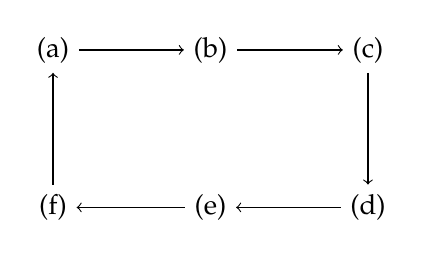
\begin{tikzpicture}[node distance=2cm] 
                % Nodes
                \node (a) {(a)};
                \node[right of=a] (b) {(b)};
                \node[right of=b] (c) {(c)};
                \node[below of=c] (d) {(d)};
                \node[below of=b] (e) {(e)};
                \node[below of=a] (f) {(f)};

                % Arrows
                \draw[->] (a) -- (b);
                \draw[->] (b) -- (c);
                \draw[->] (c) -- (d);
                \draw[->] (d) -- (e);
                \draw[->] (e) -- (f);
                \draw[->] (f) -- (a);
        \end{tikzpicture}
        \end{center}
            %%%%%%%%%%%%%%%%%  Sect. Preuve d'existance   %%%%%%%%%%%%%%%%%%%%%%%%%%%%%%%%%%%%%%%%%%%%%%%%%%%%%%%%%%%%%


        \section{Preuve d'existance}
        
        \paragraph{}
        La plupart des théorèmes sont sous la forme de propositions conditionnelles ou biconditionnelle. Nous avons
        vue qu'un proposition conditionnelle $P \implies  Q$ se traduit par une proposition 
        universellement quantitifiée, $\forall x \in S, P(x) \implies Q(x)$.
        \paragraph{}
        Or, pour \textbf{prouver une proposition d'existence}, il suffit de trouver un exemple qui satisfait 
        la proposition associée au théorème. Autrement dit, il faut montrer $\exists x, R(x)$ 

        \begin{Preuve}{Utilisation d'exemple pour une preuve d'existance}{}
            \textbf{Proposition} \quad Il existe un nombre premier qui est pair. 
            \vspace{1em}\\
            \textit{Preuve.} Observez que $2$ est un nombre premier pair.
        \end{Preuve}
        \section{Preuve constructive et non-constructive}
        
        \paragraph{} 
        Une preuve d'existance peut être constructive ou non constructive. La preuve d'existance constructive 
        indique qu'il existe un élément qui respecte la proposition et donne un exemple. La preuve d'existance 
        non-constructive indique simplement qu'il existe un élément qui respecte la proposition, mais ne donne pas 
        d'exemple. 

            %%%%%%%%%%%%%%%%%  Sect. Réfutations           %%%%%%%%%%%%%%%%%%%%%%%%%%%%%%%%%%%%%%%%%%%%%%%%%%%%%%%%%%%


        \chapter{Réfutations}
        \paragraph{}
        Le processus permettan de montrer qu'une propoisition fausse s'appelle la réfutation. Il existe trois types 
        de propositions :
        \begin{enumerate}
            \item Les propositions qui ont été prouvé. Cela inclus tous les théorèmes, lemmes, corollaires et autres 
                propositions qu'on sait vrai. 
            \item Les propositions fausses. On ne leur accorde pas de nom particulier 
                et on sait qu'elles sont fausses.
            \item Les  \textbf{conjectures} ; les propositions qu'on \textit{suspecte} être vraies, mais qui n'ont 
                pas encore été prouvées. 
        \end{enumerate}



        \paragraph{}
        Pour montrer qu'une proposition $P$ est fausse, il suffit de montrer que sa réciproque $\neg P$ est vraie, 
        puisque $P$ et $\neg P$ ne peuvent pas être vraie à la fois ; si $\neg P$ est vraie, alors $P$ est fausse.

        \section{\textcolor{myp}{\textbf{Réfutation par contre-exemple} }}
        Puisque plusieurs conjectures sont des propositions universellement quantitiées de la forme 
        $\forall x \in S, P(x)$, il suffit d'effectuer la négation : 
        \[ \neg (\forall x \in S, P(x) = \exists x \in S, \neg P(x) ) \]




            \begin{center}
            \textbf{Comment réfuter $\forall x \in S, P(x)$}  
            \\
            \noindent\fbox{%
                \parbox{0.5\linewidth}{%
                    \vspace{0.5em} % Add some vertical space
                    \noindent Produire un exemple d'un $x \in S$ \\ 
                    qui rend $P(x)$ faux. 
                    \vspace{0.25em}\\

                }%
            }
            \end{center}


            \begin{center}
            \textbf{Comment réfuter $P(x) \implies  Q(x)$}  
            \\
            \noindent\fbox{%
                \parbox{0.5\linewidth}{%
                    \vspace{0.5em} % Add some vertical space
                    \noindent Produire un exemple d'un $x$ \\ 
                    qui rend $P(x) \implies Q(x)$ faux. 
                    \vspace{0.25em}\\

                }%
            }
            \end{center}


            \begin{Definitionx}{contre-exemple}{}
                Les exemples qui réfutent une proposition sont appellés contre-exemple.
            \end{Definitionx}
            

            
            \section{\textcolor{myp}{\textbf{Réfuter les propositions d'existence}}}

            Réfuter une proposition d'existance $\exists x \in S, P(x)$ revient montrer qu'une 
            proposition universellement quantitifée est vraie :
            \[ \neg (\exists x \in S, P(x))  = \forall x \in S, P(x) \]

            %%%%%%%%%%%%%%%%%  Sect. Réfuter par contradiction %%%%%%%%%%%%%%%%%%%%%%%%%%%%%%%%%%%%%%%%%%%%%%%%%%%%%%%%


            \section{\textbf{\textcolor{myb}{Réfutation par contradiction}}}
            Supposon qu'on veut réfuter $P$. Il faut alors montrer que $\neg P$ est vrai. Or, si on procède par 
            contradiction, on va supposer que la proposition $\neg P$ est fausse, ce qui revient à 
            assumer que $\neg \neg P$ est vrai. Or, $\neg \neg P$ est simplement $P$. 
            Donc, pour réfuter par contradiction, il suffit d'assumer que $P$ est 
            vrai et déduire une contradiction. 



            \begin{center}
            \textbf{Comment réfuter $P$ par contradiction}  
            \\
            \noindent\fbox{%
                \parbox{0.9\linewidth}{%
                    \vspace{0.5em} % Add some vertical space
                    Assumer que $P$ est vraie, et déduire une \textit{contradiction}.

                }%
            }
            \end{center}


            \begin{Lemme}{Lemme d'Euclide}{}
                Si un nombre premier $k$ divise un produit $A = a_1 \cdot a_2 \dots \cdot a_n$, alors, $k$ divise 
                au moins une des facteurs de $A$. 
            \end{Lemme}

            \begin{Lemme}{Factorisation en nombre premer}{}
                Si $p$ est un nombre premier et $p|q$, alors $p$ est un facteur premier de $q$. Autrement dit, 
                la factorisation en nombre premier de $q$ implique $p$. 
                
            \end{Lemme}
\end{multicols*}
\end{document}
